\chapter{Implementasi, Pengujian, dan Eksperimen}

\section{Deskripsi Perangkat Keras dan Lunak yang Digunakan}
\label{sec:desc_perangkat}
Pembangunan perangkat lunak pada skripsi ini dilakukan dengan menggunakan aplikasi perangkat lunak \textit{IntelliJ IDEA Ultimate} 2017.1. Semua kode ditulis dengan menggunakan bahasa pemrograman \textit{Java}. \textit{Framework Hadoop} yang digunakan adalah Hadoop versi 2.7.2. Hadoop dipasang pada 5 komputer dengan spesifikasi sebagai berikut:
\begin{itemize}
	\item Sistem Operasi: Ubuntu 14.04 LTS
	\item Tipe SO: 64-bit
	\item Prosesor: Intel® Core™ i3 CPU 550 @ 3.20GHz × 4 
	\item Memori: 7,7 GiB
	\item Grafik: Gallium 0.4 on AMD REDWOOD
	\item Disk: 264,2 GB
\end{itemize}
Sebuah komputer dijadikan \textit{master} dan sisanya dijadikan sebagai \textit{slave}.

\section{Implementasi Antarmuka}
\label{sec:impl_antarmuka}

Antarmuka yang dibangun pada keseluruhan perangkat lunak ada 2 jenis. (1) Antarmuka perangkat lunak jenis pertama diperuntukkan untuk modul yang berbasis \textit{MapReduce}, dirancang dengan antarmuka \textit{shell}. (2) Antarmuka perangkat lunak jenis kedua diperuntukkan untuk modul yang tidak berbasiskan \textit{MapReduce}, seperti modul kelola input dan klasifikasi. Antarmuka pada jenis kedua ini akan dirancang menggunakan antarmuka berbasis web HTML.

\subsection{\textit{Shell}}
Perangkat lunak pada modul berbasis \textit{MapReduce} yang sudah di-\textit{compile} dengan java dalam bentuk jar akan dijalankan melalui \textit{shell} pada \textit{terminal} dengan perintah:
\begin{lstlisting}
:~$ hadoop jar MapReduce.jar /bayes/<model-directory>
\end{lstlisting}
Perintah ini akan menerima 1 buah parameter yang akan menentukan model dari direktori yang akan digunakan untuk proses \textit{MapReduce} yang akan dijalankan. Parameter tersebut memiliki \textit{namespace} yang perlu selalu diikutsertakan untuk menentukan model direktori pada saat menjalankan program, yaitu namespace \texttt{/bayes/}. Setelah \texttt{/bayes/}, kata berikutnya merupakan nama model direktori yang akan digunakan untuk menjalankan program. Misalnya, akan menjalankan program pada model bernama \texttt{car}, maka perintah yang perlu dijalankan adalah:
\begin{lstlisting}
:~$ hadoop jar MapReduce.jar /bayes/car
\end{lstlisting}
Berikut ini merupakan contoh yang salah:
\begin{lstlisting}
:~$ hadoop jar MapReduce.jar /car
\end{lstlisting}

Untuk mengingatkan penggunaan program, perlu diingat kembali urutan yang perlu dilakukan untuk menjalankan keseluruhan perangkat lunak dengan benar pada \textit{modul specification} Figure~\ref{fig:Modul Specification}. 

Di dalam model direktori yang dijadikan parameter saat menjalankan program menggunakan \textit{shell}, sudah harus memiliki beberapa direktori yang diproses pada modul kelola input, direktori serta isinya. Berikut merupakan contoh isi dalam model direktori minimal yang dibutuhkan untuk menjalankan perangkat lunak berbasis \textit{MapReduce} dengan menjalankan perintah untuk melihat seluruh isi direktori dan file secara rekursif:
\begin{lstlisting}
:~$ hadoop fs -ls -R /bayes/car
drwxrwxr-x   - hduser supergroup          0 2017-04-19 22:17 /bayes/car/info
-rw-r--r--   3 hduser supergroup        117 2017-04-19 22:17 /bayes/car/info/meta.info
drwxrwxr-x   - hduser supergroup          0 2017-04-19 22:17 /bayes/car/input
-rw-r--r--   3 hduser supergroup  569163610 2017-04-19 22:29 /bayes/car/input/dataset-1_19-04-2017_10-17.in
drwxrwxr-x   - hduser supergroup          0 2017-04-19 22:17 /bayes/car/testing
drwxrwxr-x   - hduser supergroup          0 2017-04-19 22:17 /bayes/car/testing/input
-rw-r--r--   3 hduser supergroup  232561301 2017-04-19 22:29 /bayes/car/testing/input/dataset-1_19-04-2017_10-17.in
\end{lstlisting}

\subsection{Berbasis Web HTML}
Antarmuka pada modul klasifikasi dan modul kelola input dibuat dengan menggunakan antarmuka berbasis web yaitu HTML. Seperti yang telah dijelaskan pada bagian~\ref{sec:Perancangan Antarmuka}, pada modul yang tidak berbasiskan \textit{MapReduce} ini, memiliki 6 buah antarmuka dan 1 layout untuk menu yang akan disimpan disamping kiri dari keseluruhan tampilan antarmuka.

\subsubsection{Layout Menu}
Gambar~\ref{fig:Implementasi Antarmuka Layout Menu} menunjukkan antarmuka untuk tampilan layout menu yang ada pada bagian kiri seluruh tampilan antarmuka yang dibuat. Antarmuka ini dibuat untuk memudahkan user dalam melakukan perpindahan halaman antarmuka sesuai yang diinginkan oleh user.
\begin{figure}[H]
	\centering
	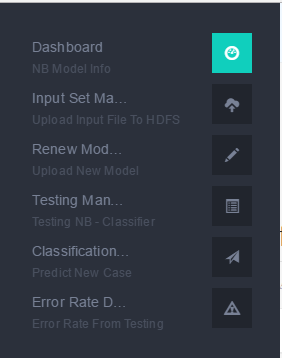
\includegraphics[scale=0.65]{ImplGUI/layout_menu}
	\caption[Implementasi Antarmuka Layout Menu]{Implementasi Antarmuka Layout Menu}
	\label{fig:Implementasi Antarmuka Layout Menu}
\end{figure}


\subsubsection{Dashboard}
Gambar~\ref{fig:Implementasi Antarmuka Dashboard} menunjukkan antarmuka tampilan awal pada modul \textit{non-MapReduce}. Seperti yang sudah dijelaskan di bagian rancangan antarmuka \textit{Dashboard} pada bagian~\ref{subsec:Dashboard}, pada tampilan ini user bisa melakukan monitor model NBC yang telah dimasukkan ke dalam perangkat lunak ini, seperti melihat seluruh atribut kelas dan atribut prediktor, lalu frekuensi kemunculan untuk setiap atribut kelas dan atribut prediktor bertipe diskrit, dan juga nilai rata - rata dan standard deviasi untuk atribut prediktor bertipe numerik. 

Terdapat keterangan dari nama kolom pada bagian \textit{Bayesian Model} yang perlu diperhatikan. \verb|P_N = Predictor Name|; \verb|P_V = Predictor Value|; \verb|C_N = Class Name|; \verb|C_V = Class Value|.

\begin{figure}[H]
	\centering
	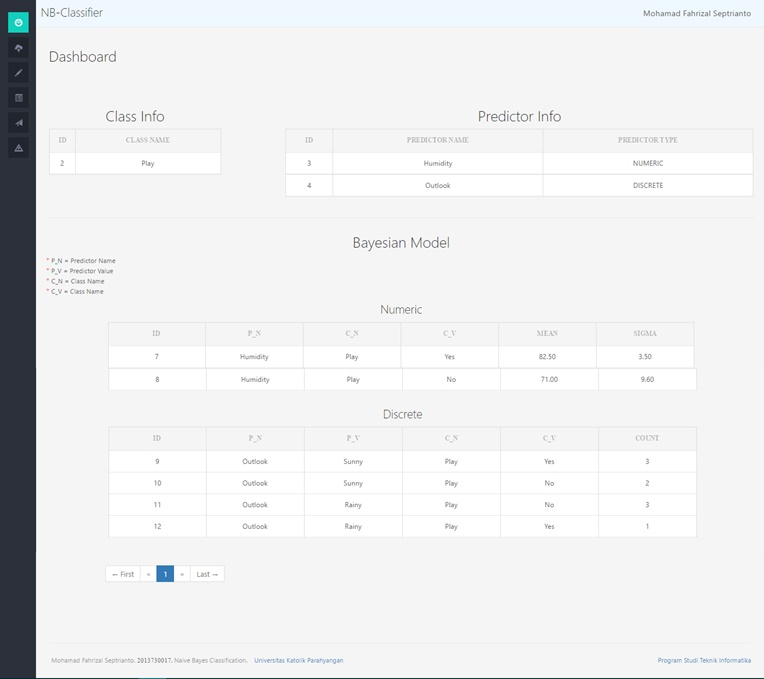
\includegraphics[scale=0.65]{ImplGUI/dashboard}
	\caption[Implementasi Antarmuka Dashboard]{Implementasi Antarmuka Dashboard}
	\label{fig:Implementasi Antarmuka Dashboard}
\end{figure}


\subsubsection{Input Set Manager}
Gambar~\ref{fig:Implementasi Antarmuka Input Set Manager} menunjukkan antarmuka untuk melakukan pengelolaan file input untuk ditransfer ke dalam HDFS yang nantinya akan menjadi file untuk data latih dan data testing algoritma klasifikasi \textit{naive bayes}. Seperti yang sudah dijelaskan di bagian rancangan antarmuka \textit{Input Set Manager} pada~\ref{subsec:Input Set Manager}, bahwa user dapat memilih model direktori; user dapat memilih file input dan file info; user dapat memilih presentase penggunaan file input untuk dijadikan data \textit{training} dan data \textit{testing}; user dapat memilih penggunaan dan jenis setiap atribut pada file yang di-input-kan oleh user.

\begin{figure}[H]
	\centering
	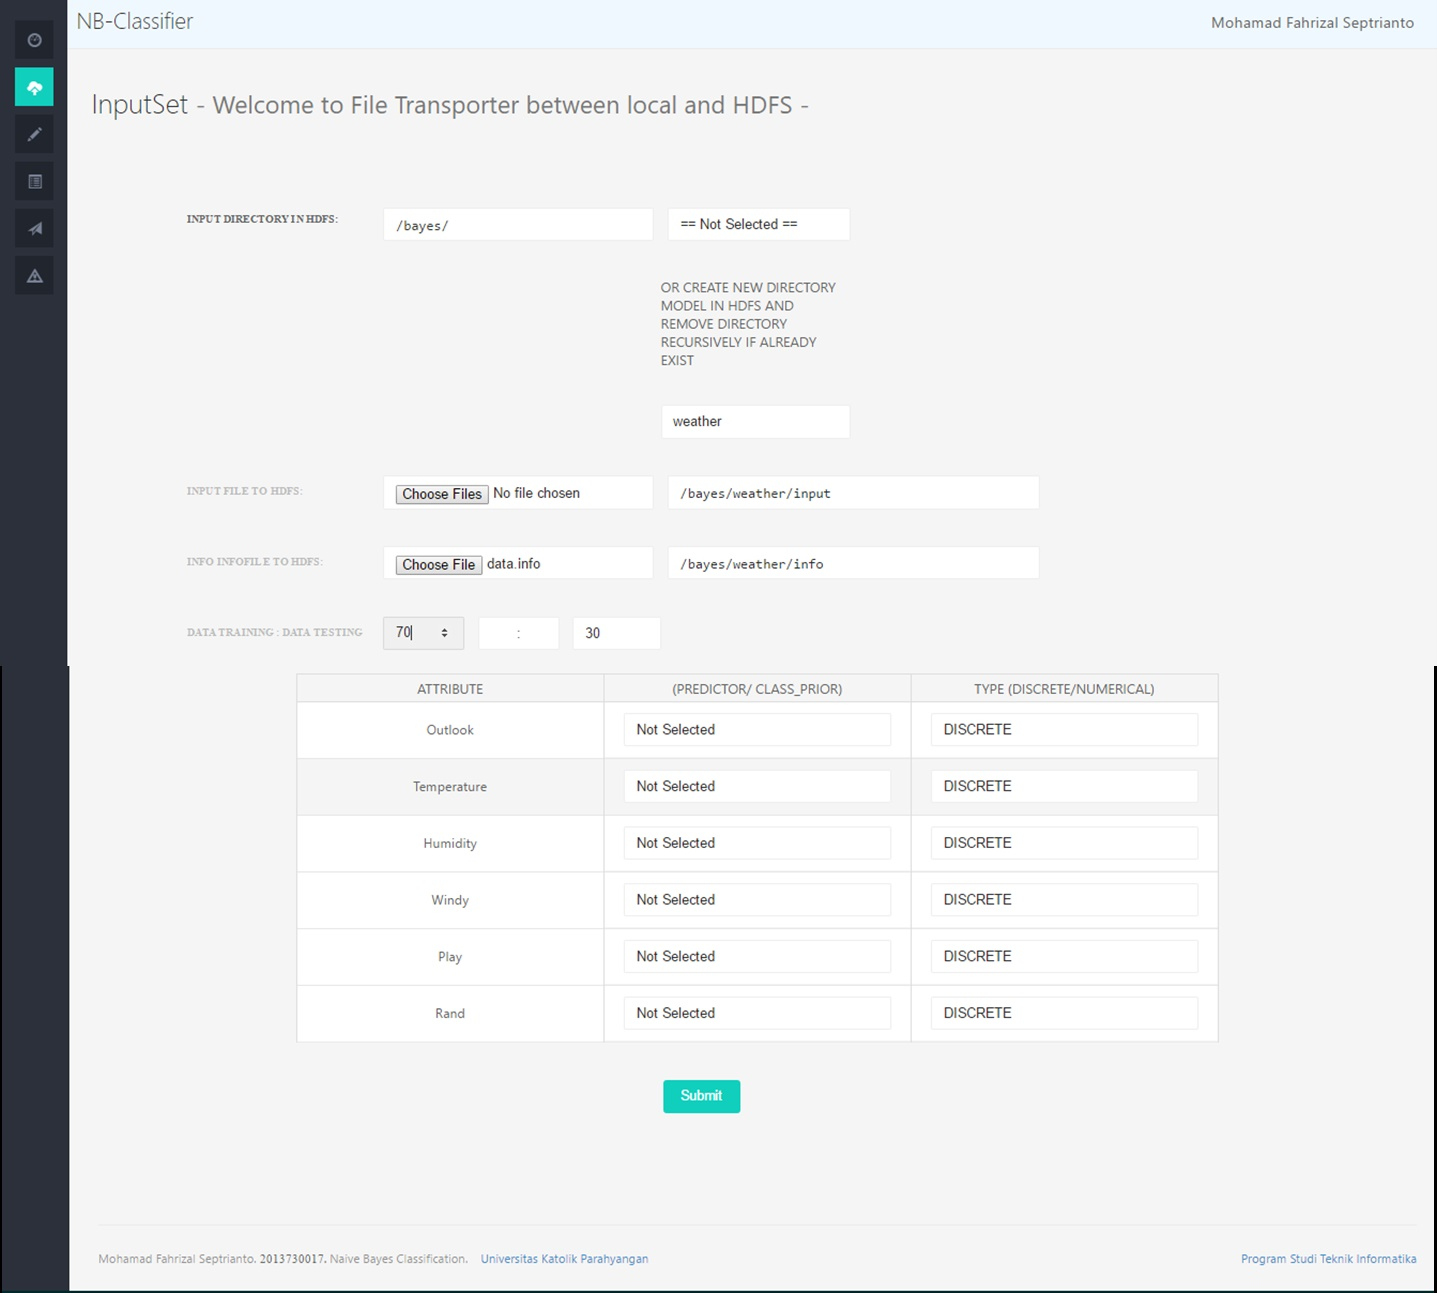
\includegraphics[scale=0.4]{ImplGUI/input}
	\caption[Implementasi Antarmuka Input Set Manager]{Implementasi Antarmuka Input Set Manager}
	\label{fig:Implementasi Antarmuka Input Set Manager}
\end{figure}


\subsubsection{Renew Model Manager}
Gambar~\ref{fig:Implementasi Antarmuka Renew Model Manager} menunjukkan antarmuka untuk melakukan pembaharuan model NBC pada perangkat lunak untuk melakukan testing dan klasifikasi pada modul yang berbasis \textit{non-MapReduce}. Seperti yang sudah dijelaskan di bagian perancangan antarmuka \textit{Renew Model Manager} pada bagian~\ref{subsec:Renew Model Manager}, user bisa melakukan pembaharuan model NBC dari penyimpanan local milik user, atau langsung dari model direktori yang berada di dalam HDFS.

\begin{figure}[H]
	\centering
	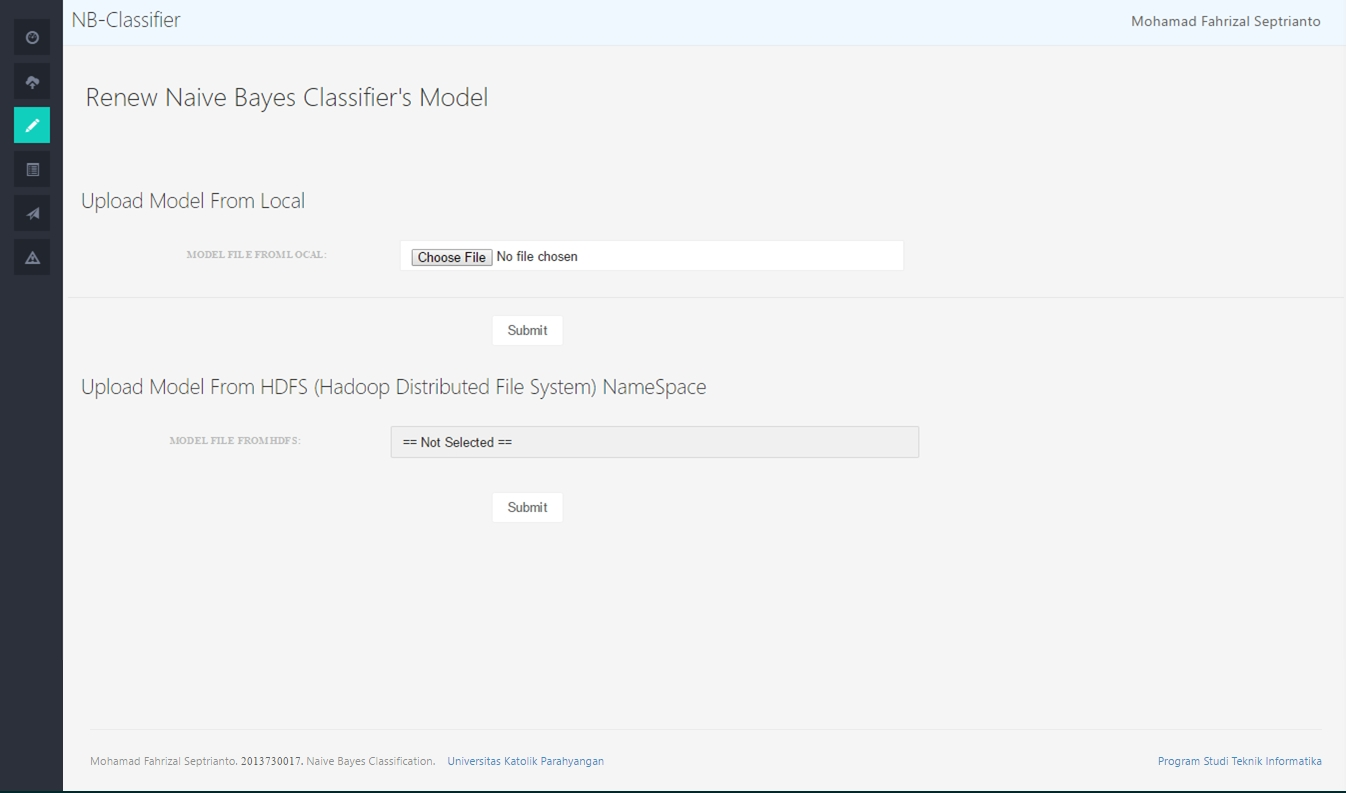
\includegraphics[scale=0.45]{ImplGUI/renewmodel}
	\caption[Implementasi Antarmuka Renew Model Manager]{Implementasi Antarmuka Renew Model Manager}
	\label{fig:Implementasi Antarmuka Renew Model Manager}
\end{figure}


\subsubsection{Testing Manager}
Gambar~\ref{fig:Implementasi Antarmuka Testing Manager} menunjukkan antarmuka untuk melakukan testing pada model NBC yang sudah ada di dalam program sebelumnya. Seperti yang sudah dijelaskan di bagian perancangan antarmuka \textit{Testing Manager} pada bagian~\ref{subsec:Testing Manager}, user dapat melakukan testing menggunakan data testing yang berada pada penyimpanan local milik user, atau melalui data testing yang sudah ada pada model direktori dalam HDFS.

\begin{figure}[H]
	\centering
	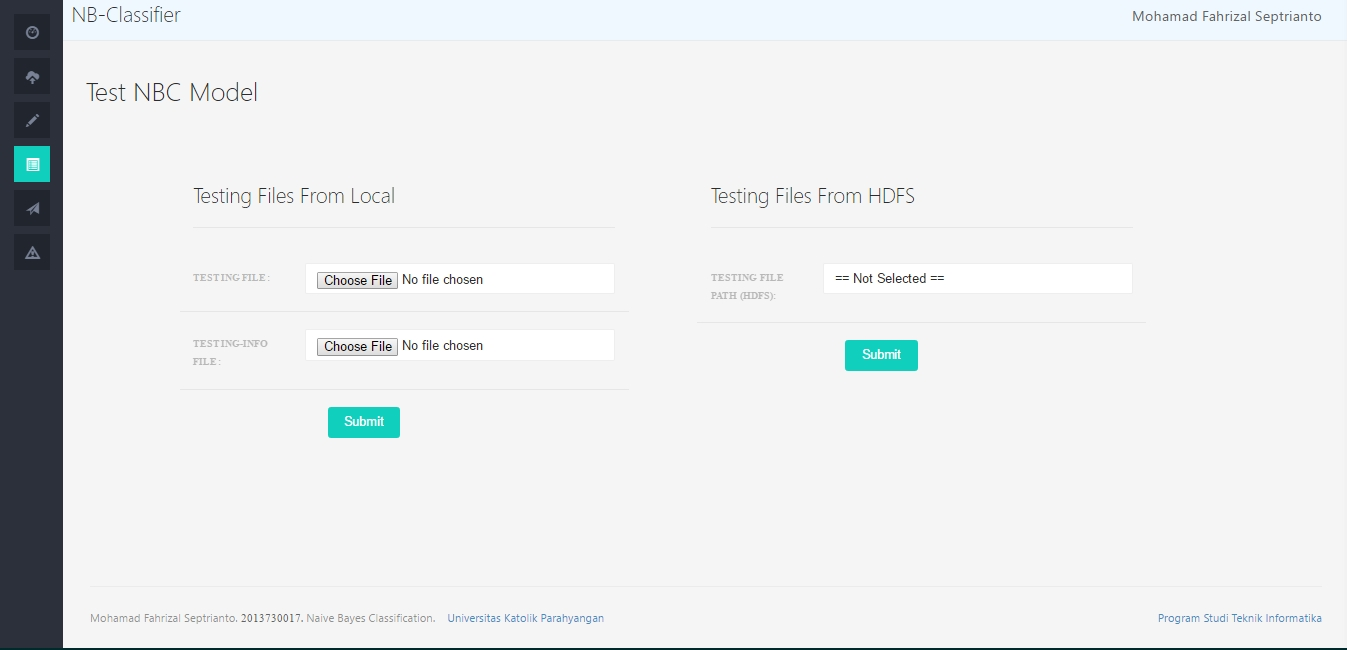
\includegraphics[scale=0.45]{ImplGUI/testing}
	\caption[Implementasi Antarmuka Testing Manager]{Implementasi Antarmuka Testing Manager}
	\label{fig:Implementasi Antarmuka Testing Manager}
\end{figure}

\subsubsection{Classification Manager}
Gambar~\ref{fig:Implementasi Antarmuka Classification Manager} menunjukkan antarmuka untuk melakukan klasifikasi pada model NBC(\textit{single case prediction}). Seperti yang sudah dijelaskan di bagian perancangan antarmuka \textit{Classification Manager} pada bagian~\ref{subsec:Classification Manager}, user dapat melakukan input manual untuk 1 kasus baru dengan mengisi nilai atribut prediktor yang dibutuhkan dan atribut kelas (\textit{optional}) yang nantinya akan diumpankan ke dalam model NBC untuk dilakukan klasifikasi.

\begin{figure}[H]
	\centering
	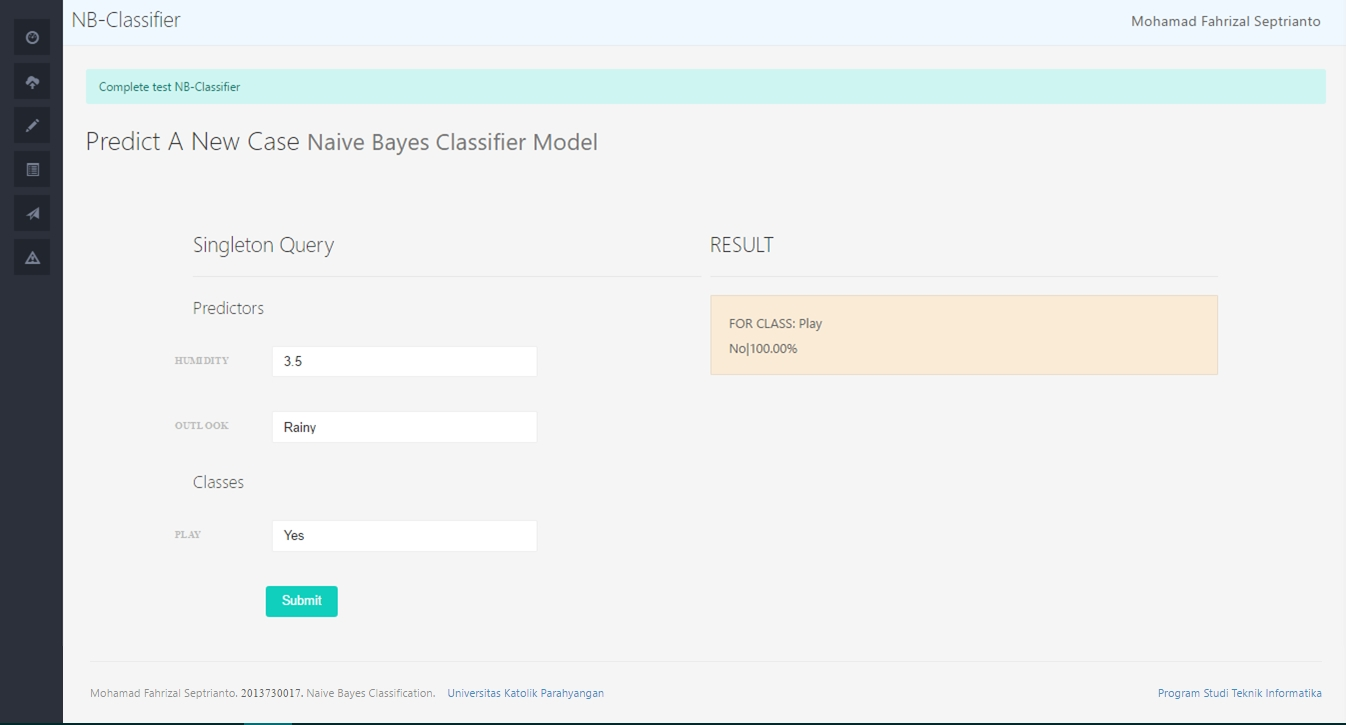
\includegraphics[scale=0.425]{ImplGUI/classification}
	\caption[Implementasi Antarmuka Classification Manager]{Implementasi Antarmuka Classification Manager}
	\label{fig:Implementasi Antarmuka Classification Manager}
\end{figure}

\subsubsection{Error Rate Dashboard}
Gambar~\ref{fig:Implementasi Antarmuka Error Rate Dashboard} menunjukkan antarmuka untuk melakukan monitor terhadap nilai - nilai \textit{error rate} yang muncul setelah melakukan testing terhadap model NBC. Seperti yang sudah dijelaskan di bagian perancangan antarmuka \textit{Error Rate Dashboard} pada bagian~\ref{subsec:Error Rate Dashboard}, user dapat melakukan monitor terhadap matrix \textit{confusion} yang dihasilkan dan juga beberapa nilai - nilai \textit{error rate} yang dihasilkan. Selain itu, untuk mengingatkan user kepada formula - formula yang digunakan untuk menghasilkan nilai \textit{error rate}, pada bagian paling bawah antarmuka juga menampilkan formula - formula yang digunakan dalam menghasilkan tiap nilai \textit{error rate} yang digunakan. 

\begin{figure}[H]
	\centering
	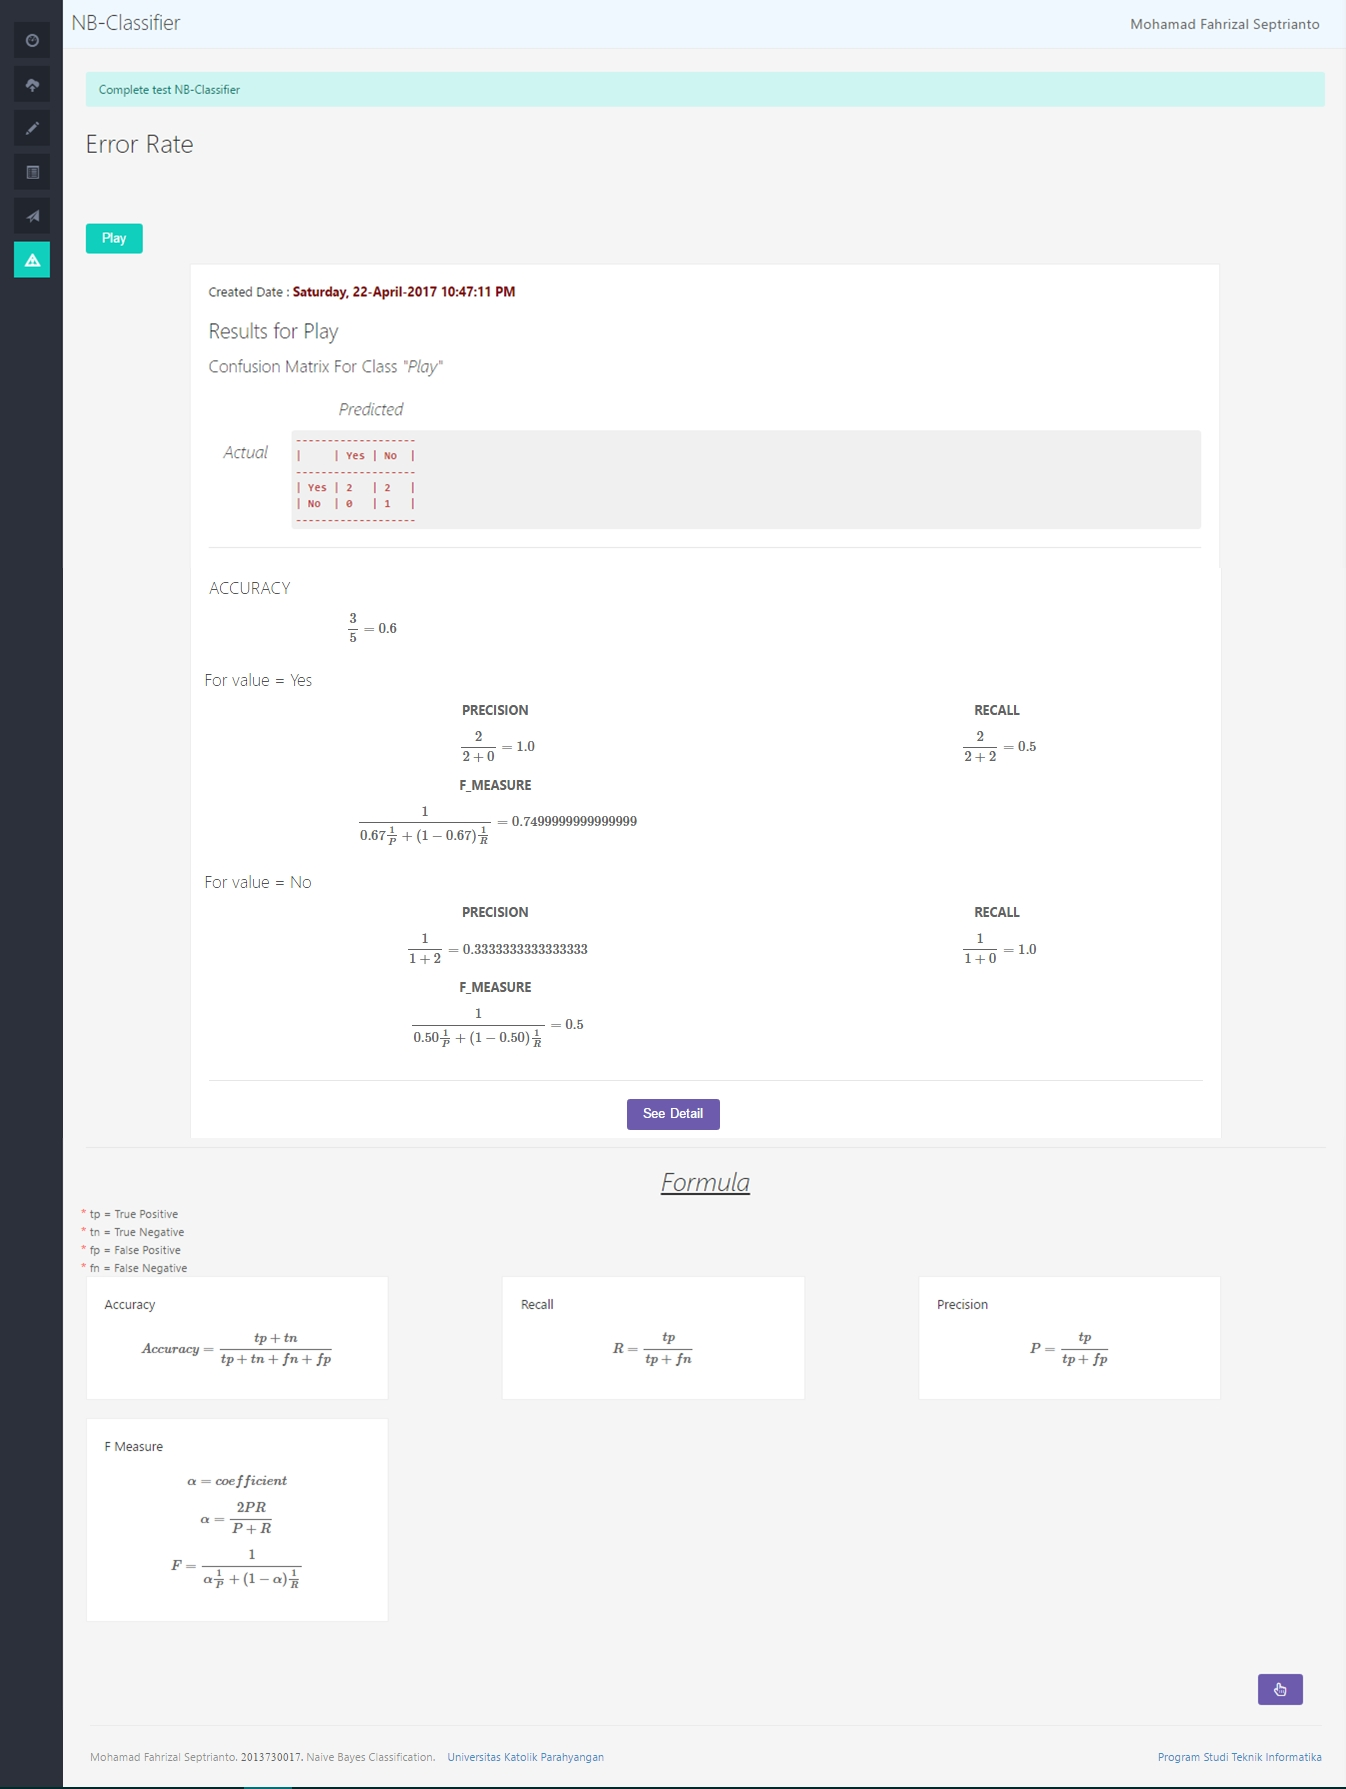
\includegraphics[scale=0.45]{ImplGUI/error_rate}
	\caption[Implementasi Antarmuka Error Rate Dashboard]{Implementasi Antarmuka Error Rate Dashboard}
	\label{fig:Implementasi Antarmuka Error Rate Dashboard}
\end{figure}

\section{Implementasi Package, Kelas, dan Method dengan Java}
\label{sec:impl_code}

Implementasi untuk setiap modul dari kelas-kelas dan method-method hasil dari analisis dan rancangan pada bahasa pemrograman Java yang dikelompokan berdasarkan Package, dicantumkan dan dapat dilihat pada lampiran - lampiran sebagai berikut:
\begin{enumerate}
	\item Modul \textit{Training Naive Bayes M-R Based} berada pada lampiran~\ref{lamp:A}
	\item Modul \textit{Testing Naive Bayes M-R Based} berada pada lampiran~\ref{lamp:B}
	\item Modul Kelola Input dan Klasifikasi berbasis \textit{non-MapReduce} berapa pada lampiran~\ref{lamp:C}
\end{enumerate}

\section{Pengujian Kebenaran}
Bagian ini akan menunjukkan pengujian kebenaran terhadap perangkat lunak yang dibangun dengan membandingkan perhitungan manual yang akan dilakukan pada bagian~\ref{subsec:Perhitungan Manual Dengan Data Studi Kasus} dengan perhitungan dengan menggunakan program pada bagian~\ref{subsec:Perhitungan Menggunakan Perangkat Lunak yang Dibangun Dengan Data Studi Kasus} dengan data yang sama. Data yang digunakan pada kedua perhitungan tersebut merupakan data yang sama. Data studi kasus diperoleh dengan cara mengambil dari situs \url{http://cse-wiki.unl.edu/wiki/images/e/e0/Golf_dataset.png} yang diambil pada pada 23 April 20117, dan telah dilakukan modifikasi sedikit terhadap data agar menjadi lebih simpel.

\subsection{Perhitungan Manual Dengan Data Studi Kasus}
\label{subsec:Perhitungan Manual Dengan Data Studi Kasus}
Pada bagian ini akan dilakukan perhitungan manual dengan menggunakan data studi kasus yang menunjukkan seseorang akan bermain tenis atau tidak berdasarkan dari data kelembaban dari cuaca dan pemandangan yang terjadi.

\subsubsection{Pembuatan Model NBC}
%\subsubsection{Tahapan Membuat Model Klasifikasi Dari Algoritma Naive Bayes}		
Misal kita memiliki dataset yang menunjukan seseorang akan bermain tenis atau tidak berdasarkan dari data kelembaban dan pemandangan yang terjadi seperti pada Tabel~\ref{tab:dataset} berikut: 
		
		\begin{table}[H]
		\label{tab:dataset}
		\centering
		\caption{Contoh Dataset (atribut kelas = \textbf{Play})}
		\begin{tabular}{ | c | c | c | }
		\hline
		%\toprule
		 Humidity & Outlook & \textbf{Play}\\ \hline \hline
		%\midrule
		60 & Rainy & No\\ \hline
		%\midrule
		78 & Rainy & No\\ \hline
		%\midrule
		80 & Sunny & Yes\\ \hline
		%\midrule
		75 & Sunny & No\\ \hline
		%\midrule
		85 & Sunny & Yes \\ \hline
		%\bottomrule
		\end{tabular}
		\end{table}
		
		
		Langkah pertama yang perlu dilakukan untuk membuat algoritma naive bayes classifier adalah membuat table frekuensi untuk setiap atribut prediktor terhadap atribut kelas yang bertipe Diskrit. Pada contoh tabel diatas, diasumsikan bahwa atribut Humidity dan Outlook merupakan atribut prediktor, lalu untuk atribut Play merupakan atribut kelas.
		
		\begin{table}[ht]
			\centering
			\caption{Table frekuensi atribut Outlook}
			\begin{tabular}{ | c | c | c | c | }
			\hline
			 & \multicolumn{2}{c}{\textbf{Play}} & \\ 
			%\hline
			 & Yes & No & \textit{sum} \\
			\hline
			Sunny & 2 & 1 & \textbf{3}\\
			\hline
			Rainy & 0 & 2 & \textbf{2} \\
			\hline
			\textit{sum} & \textbf{2} & \textbf{3} & \\
			\hline
			\end{tabular}
		\end{table}
		
		Pada table frekuensi untuk atribut Outlook, dapat dilihat bahwa $P(X=Rainy|C=Yes) = 0$. Naive bayes classifier tidak dapat mengatasi frekuensi yang nilainya 0. Karena dapat menyebabkan seluruh perhitungan menjadi 0(karena berapapun bilangannya, jika dikalikan dengan 0 akan selalu menghasilkan nilai 0), sehingga menjadi tidak relevan. Pendekatan yang perlu digunakan untuk mengatasi hal tersebut adalah dengan menggunakan metode Laplacian Correction (->Pustaka.Bib). Pada metode tersebut, dikatakan bahwa kita perlu menambah nilai 1 kepada seluruh nilai pada table frekuensi untuk mengatasi masalah \textit{zero-frequency problems}. Asumsikan training database (D) itu sangat besar, dimana menambahkan frekuensi sebanyak 1 ke setiap jumlah perhitungan yang kita perlukan tidak akan memberikan pengaruh yang besar terhadap nilai kemungkinan akhir (Laplacian correction / Laplace estimator) \cite{PeughMissing:2004}. Perubahan nilai atribut dapat dilihat pada table 3. \\
		
		\begin{table}[ht]
			\centering
			\caption{Table frekuensi atribut Outlook}
			\begin{tabular}{|c|c|c|c|}
			\hline
			 & \multicolumn{2}{c}{\textbf{Play}} & \\
			 & Yes & No & \textit{sum} \\ 
			\hline
			Sunny & 3 & 2 & \textbf{5}\\
			\hline
			Rainy & 1 & 3 & \textbf{4} \\
			\hline
			\textit{sum} & \textbf{4} & \textbf{5} & \\
			\hline
			\end{tabular}
		\end{table}
		
		
		Langkah kedua adalah membuat table kemungkinan dari table frekuensi yang telah dibuat :		
		\begin{table}[ht]
			\centering
			\caption{Table kemungkinan atribut Outlook}
			\begin{tabular}{|c|c|c|c|}
			\toprule
			 & \multicolumn{2}{c}{\textbf{Play}} & \\
			 & Yes & No & \textit{sum} \\ 
			\midrule
			Sunny & 3/4 & 2/5 & \textbf{5/9}\\
			\midrule
			Rainy & 1/4 & 3/5 & \textbf{4/9} \\
			\midrule
			\textit{sum} & \textbf{4/9} & \textbf{5/9} & \\
			\bottomrule
			\end{tabular}
		\end{table}
		
		Karena atribut Humidity bertipe numerik, atribut tersebut perlu diubah ke dalam kategori mereka masing - masing agar perhitungan dalam pembuatan model dapat tepat. Konversi atribut yang bertipe numerik bisa menggunakan distribusi variabel numerik untuk dapat menebak frekuensi-nya dengan mengasumsikan distribusi normal untuk variabel numerik. Rumus yang digunakan adalah :\\
		
		\textbf{Mencari mean (rata - rata)} 
		\begin{equation}
			\mu = \dfrac{1}{n} \mathlarger{\mathlarger{\sum}}_{i=1}^{n}x_i
		\end{equation}
		
		\textbf{Mencari Standard Deviation}
		\begin{equation}
			\sigma = \mathlarger{[ \dfrac{1}{n - 1} * \mathlarger{\mathlarger{\sum}}_{i=1}^{n} (x_i - \mu)^2]}^{0.5}
		\end{equation}
		
		\textbf{Normal Distribution}
		\begin{equation}
			f(x) = \dfrac{1}{\sqrt{2\pi\sigma}}e^{-\dfrac{(x-\mu)^2}{2\sigma^2}}
		\end{equation}
		
		Berikut merupakan table rata - rata dan standar deviasi dari atribut Humidity yang bertipe numerik : 
		
		\begin{table}[h]
		\centering
		\caption{Table rata - rata dan standar deviasi atribut Humidity}
		\begin{tabular}{|c|c|c|c|c|}
		\toprule
		\multirow{2}{*}{Play Golf ?} & Yes & 80 & 85 & \\
		 & No & 60 & 75 & 78 \\
		\bottomrule
		\end{tabular}
		\end{table}
		
		\begin{table}[ht]
		\centering
		\caption{Table Distribusi}
		\begin{tabular}{|c|c|c|}
		\toprule
		 & Mean & StDev \\
		Yes & 82.5 & 3.5 \\
		No & 71 & 9.6 \\
		\bottomrule
		\end{tabular}
		\end{table}
		
		Dari table distribusi tersebut didapatkan formula untuk menghitung klasifikasi untuk atribut Humidity adalah:
		
		\begin{equation}
			%f(x|play=yes) = \dfrac{1}{\sqrt{2\pi(3.5)}}e^{-\dfrac{(x-82.5)^2}{2(3.5)^2}} 
			f(x|play=yes) = \dfrac{1}{\sqrt{2\pi(3.5)}}e^{-\dfrac{(x-82.5)^2}{2(3.5)^2}}
		\end{equation}
		\begin{equation}
			f(x|play=no) = \dfrac{1}{\sqrt{2\pi(9.6)}}e^{-\dfrac{(x-71)^2}{2(9.6)^2}} 
		\end{equation}
		
		\textit{Cara ini dapat diberlakukan juga pada atribut yang bertipe kontinu.}
		
		Setelah semua model dari naive bayes classifier telah jadi, maka klasifikasi sudah dapat dilakukan dengan model diatas.

\subsubsection{Klasifikasi Menggunakan Model NBC}
%\subsection{Contoh perhitungan klasifikasi algoritma naive bayes}		
		Dimisalkan kita memiliki 2 buah dataset yang akan diuji menggunakan model klasifikasi yang telah dibangun sebelumnya, seperti berikut :
		
\begin{enumerate}
	\item $X = {Humidity = 50, Outlook = Sunny}$
	\item $Y = {Humidity = 90, Outlook = Sunny}$
\end{enumerate}
		
Untuk dataset X dan Y, akan dicari peluang kelas yang paling tinggi. \\
		
$( C_{MAP} = \underset{c \in C}{ argmax } P(c|d) = \underset{c \in C}{ argmax } \dfrac{P(d|c) P(c)}{P(d)} = \underset{c \in C}{ argmax } P(d|c) P(c) )$
		
\paragraph{Untuk dataset X dengan $P=Yes$:}
	Menghitung peluang untuk atribut $Outlook=Sunny$ dengan $P=Yes$
	\begin{equation}
			P(Outlook=Sunny|Yes) = 3/4 
			= 0.75
	\end{equation}
	
	Menghitung peluang untuk atribut $Humidity=50$ dengan $P=Yes$
		\begin{equation}
			P(Humidity=50|Yes) 
			= \dfrac{1}{\sqrt{2\pi(3.5)}}e^{-\dfrac{(\textbf{50}-82.5)^2}{2(3.5)^2}}
			= 4.031
		\end{equation}
	
	\paragraph{Untuk dataset X dengan $P=No$:}
		Menghitung peluang untuk atribut $Outlook=Sunny$ dengan $P=No$
		\begin{equation}
			P(Outlook=Sunny|No) = 2/5 
			= 0.4
		\end{equation}
		Menghitung peluang untuk atribut $Humidity=50$ dengan $P=No$
		\begin{equation}
			P(Humidity=50|No) 
			= \dfrac{1}{\sqrt{2\pi(9.6)}}e^{-\dfrac{(\textbf{50}-71)^2}{2(9.6)^2}}
			= 0.011
		\end{equation}
	\paragraph{Kesimpulan untuk $dataset$ $X$}
	Dari perhitungan di atas, didapat bahwa : \\ \\
	Untuk kelas $Play=Yes$ \\
	$P(Play=Yes|X) \\
	= P(Outlook=Sunny|Play=Yes)*P(Humidity=50|Play=Yes)*P(Yes) \\
	= 0.75 * 4.031 * 4/9 \\
	= 1.343$ \\ \\
	Untuk kelas $Play=No$ \\
	$P(Play=No|X) \\
	= P(Outlook=Sunny|Play=No)*P(Humidity=50|Play=No)*P(No) \\
	= 0.4 * 0.011 * 5/9 \\
	= 0.002$ \\ \\
	Setelah itu, lakukan normalisasi terhadap nilai - nilai berikut: \\
	$P(Play=Yes|X) = 1.343 / (1.343+0.002) \\
	= 0.998 (99.8\%)$ \\
	$P(Play=No|X) = 0.002 / (1.343+0.002) \\
	= 0.002 (0.2\%)$ \\
	
	Karena, $P(Play=Yes|X) > P(Play=No|X)$, maka hasil klasifikasi untuk \textit{dataset X} ialah kelas $Play=Yes$.
	
	\paragraph{Untuk dataset Y dengan $P=Yes$:}
	Menghitung peluang untuk atribut $Outlook=Sunny$ dengan $P=Yes$
	\begin{equation}
			P(Outlook=Sunny|Yes) = 3/4 
			= 0.75
	\end{equation}
	
	Menghitung peluang untuk atribut $Humidity=90$ dengan $P=Yes$
		\begin{equation}
			P(Humidity=90|Yes) 
			= \dfrac{1}{\sqrt{2\pi(3.5)}}e^{-\dfrac{(\textbf{90}-82.5)^2}{2(3.5)^2}}
			= 0.021
		\end{equation}
	
	\paragraph{Untuk dataset Y dengan $P=No$:}
	Menghitung peluang untuk atribut $Outlook=Sunny$ dengan $P=No$
	\begin{equation}
				P(Outlook=Sunny|No)
				= 2/5 
				= 0.4
		\end{equation}
	
	Menghitung peluang untuk atribut $Humidity=90$ dengan $P=No$
		\begin{equation}
			P(Humidity=90|No)
			= \dfrac{1}{\sqrt{2\pi(9.6)}}e^{-\dfrac{(\textbf{90}-71)^2}{2(9.6)^2}} 
			= 0.018
		\end{equation}
		
	\paragraph{Kesimpulan untuk $dataset$ $Y$}
	Dari perhitungan di atas, didapat bahwa : \\ \\
	Untuk kelas $Play=Yes$ \\
	$P(Play=Yes|Y) \\
	= P(Outlook=Sunny|Play=Yes)*P(Humidity=90|Play=Yes)*P(Yes) \\
	= 0.75 * 0.021 * 4/9 \\
	= 0.007$ \\ \\
	Untuk kelas $Play=No$ \\
	$P(Play=No|Y) \\
	= P(Outlook=Sunny|Play=No)*P(Humidity=90|Play=No)*P(No) \\
	= 0.4 * 0.018 * 5/9 \\
	= 0.004$ \\ \\
	Setelah itu, lakukan normalisasi terhadap nilai - nilai berikut: \\
	$P(Play=Yes|Y) = 0.007 / (0.007+0.004) \\
	= 0.64 (64\%)$ \\
	$P(Play=No|Y) = 0.004 / (0.007+0.004) \\
	= 0.46 (46\%)$ \\
	
	Karena, $P(Play=Yes|Y) > P(Play=No|Y)$, maka hasil klasifikasi untuk \textit{dataset Y} ialah kelas $Play=Yes$.
	

\subsection{Perhitungan Menggunakan Perangkat Lunak yang Dibangun Dengan Data Studi Kasus}
\label{subsec:Perhitungan Menggunakan Perangkat Lunak yang Dibangun Dengan Data Studi Kasus}

Pada bagian ini akan dilakukan perhitungan manual dengan menggunakan data studi kasus yang menunjukkan seseorang akan bermain tenis atau tidak berdasarkan dari data kelembaban dari cuaca dan pemandangan yang terjadi.

\subsubsection{Pembuatan model NBC}
\label{subsubsec:Pembuatan model naive bayes classifier}

Untuk dataset seperti berikut:
\begin{table}[H]
\label{tab:dataset-pl}
\centering
\caption{Contoh Dataset (atribut kelas = \textbf{Play})}
\begin{tabular}{ | c | c | c | }
\hline
%\toprule
	Humidity & Outlook & \textbf{Play}\\ \hline \hline
%\midrule
60 & Rainy & No\\ \hline
%\midrule
78 & Rainy & No\\ \hline
%\midrule
80 & Sunny & Yes\\ \hline
%\midrule
75 & Sunny & No\\ \hline
%\midrule
85 & Sunny & Yes \\ \hline
%\bottomrule
\end{tabular}
\end{table}

Akan dilakukan eksekusi program bebasis \textit{MapReduce} untuk melakukan training pembuatan model NBC dengan melakukan perintah (\textit{*diasumsikan data input telah berada pada direktori \texttt{/bayes/weather/input} di dalam HDFS}):
\begin{lstlisting}
:~$ hadoop jar mapreduce-train.jar /bayes/weather
\end{lstlisting}

Keterangan hasil output dari \textit{log} yang diterima lewat terminal setelah melakukan eksekusi program dapat dilihat pada lampiran~\ref{lamp:D}

Hasil pembuatan model klasifikasi NBC yang dilakukan oleh program dapat dilihat pada direktori \texttt{/bayes/weather/output/part-r-00000}. Hasil model tersebut adalah sebagai berikut:
\begin{lstlisting}
Play,No,3.0|CLASS	
Play,Yes,2.0|CLASS	
Humidity,Play,No	;71.0|7.874007874011811|NUMERIC
Humidity,Play,Yes	;82.5|2.5|NUMERIC
Outlook,Rainy,Play,No,2.0|DISCRETE	
Outlook,Sunny,Play,No,1.0|DISCRETE	
Outlook,Sunny,Play,Yes,2.0|DISCRETE
\end{lstlisting}

\subsubsection{Klasifikasi Menggunakan Model NBC}
Setelah model NBC diperoleh dari hasil eksekusi program \textit{train naive bayes} berbasis \textit{MapReduce} pada bagian~\ref{subsubsec:Pembuatan model naive bayes classifier}, akan dilakukan klasifikasi dan testing pada model NBC tersebut.

Pada bagian ini, akan dilakukan 2 kali pengujian klasifikasi, yaitu (1) dengan menggunakan perangkat lunak berbasis \textit{MapReduce} pada modul \textit{Testing Naive Bayes} dan (2) dengan menggunakan perangkat lunak berbasis \textit{non-MapReduce} pada modul Klasifikasi.
\begin{enumerate}
	\item{Klasifikasi dengan perangkat lunak berbasis \textit{MapReduce}}\\
	Diasumsikan data \textit{testing} untuk pengujian model NBC yang sama dengan pada perhitungan manual sudah berada pada direktori \texttt{/bayes/weather/testing/input} dalam HDFS. Program testing akan dieksekusi dengan menjalankan perintah:
	\begin{lstlisting}
	:~$ hadoop jar mapreduce-train.jar /bayes/weather
	\end{lstlisting}
	
	Keterangan hasil output dari \textit{log} yang diterima lewat terminal setelah melakukan eksekusi program dapat dilihat pada lampiran~\ref{lamp:D}.
	
	Setelah berhasil, dapat dilihat hasil dari output program pada direktori\\ \texttt{/bayes/weather/testing/output/part-r-00000}:
	\begin{lstlisting}
	@play
	####
	-------------------
	|     | no  | yes |
	-------------------
	| no  | 0   | 0   |
	| yes | 0   | 2   |
	-------------------
	####
	\end{lstlisting}
	Dapat dilihat bahwa, hasil klasifikasi menggunakan program berbasis \textit{MapReduce} pada modul \textit{testing} memiliki hasil yang sama dengan hasil klasifikasi kelas \texttt{Play=Yes}.
	
	\item{Klasifikasi dengan perangkat lunak berbasis \textit{non-MapReduce}}\\
	Model pada NBC akan di-\textit{import} ke dalam program yang dibuat dengan melakukan pembaharuan model pada antarmuka \textit{Renew Model Manager}. Program akan melakukan pembacaan terhadap model NBC dan mendeteksi dari model NBC yang diperoleh sebelumnya terdapat \textit{zero-frequency problem} dan mengatasinya dengan menggunakan metode \textit{laplacian correction}, dan hasilnya adalah seperti berikut:
	\begin{figure}[H]
	\centering
	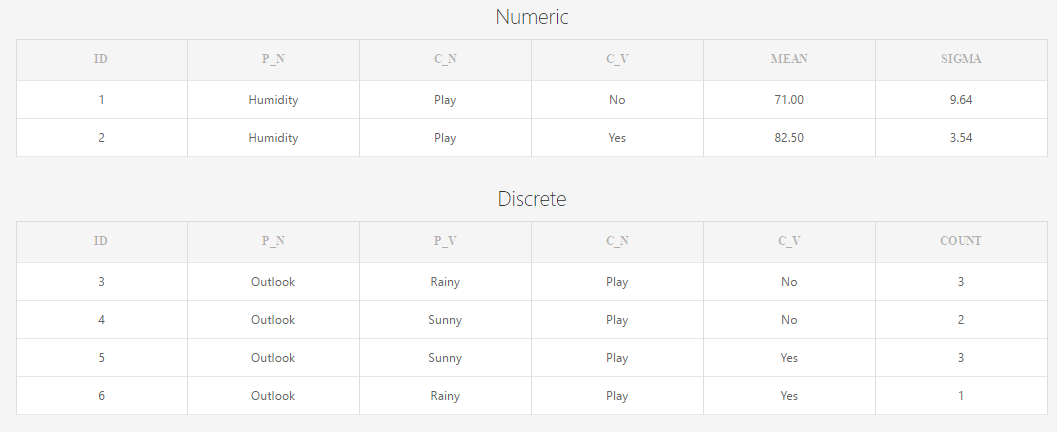
\includegraphics[scale=0.5]{Pengujian/pengujian-nonmr}
	\caption[Import Model NBC - Pengujian]{Import Model NBC - Pengujian}
	\label{fig:Import Model NBC - Pengujian}
	\end{figure}
Dapat dilihat pada Gambar~\ref{fig:Import Model NBC - Pengujian} bahwa pada model yang dihasilkan sebelumnya kita tidak memiliki frekuensi kemunculan untuk prediktor \texttt{outlook=rainy} dengan kelas \texttt{play=yes}, tetapi setelah dilakukan import model ke dalam program, program telah menangani \textit{zero-frequency problem} dengan baik, dengan menambahkan frekuensi sebanyak 1 untuk tiap model.\\

Untuk data input klasifikasi \texttt{Humidity=50} dan \texttt{Outlook=Sunny}, diperoleh hasil klasifikasi yang sama dengan perhitungan manual, yaitu kelas \texttt{Play=Yes}, dengan presentase dominasi yang berbeda sebesar \texttt{100\%}.
\begin{figure}[H]
	\centering
	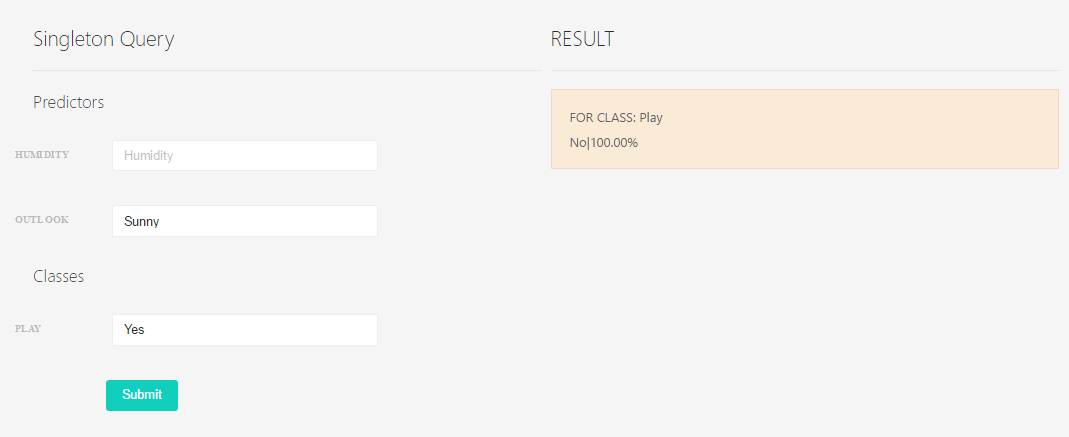
\includegraphics[scale=0.5]{Pengujian/result_classify_1}
	\caption[Hasil Klasifikasi Dataset-1]{Hasil Klasifikasi Dataset-1}
	\label{fig:Hasil Klasifikasi Dataset-1}
\end{figure}

Untuk data input klasifikasi \texttt{Humidity=90} dan \texttt{Outlook=Sunny}, diperoleh hasil klasifikasi yang sama dengan perhitungan manual, yaitu kelas \texttt{Play=Yes}, dengan presentase dominasi yang berbeda sebesar \texttt{63.94\%}.
\begin{figure}[H]
	\centering
	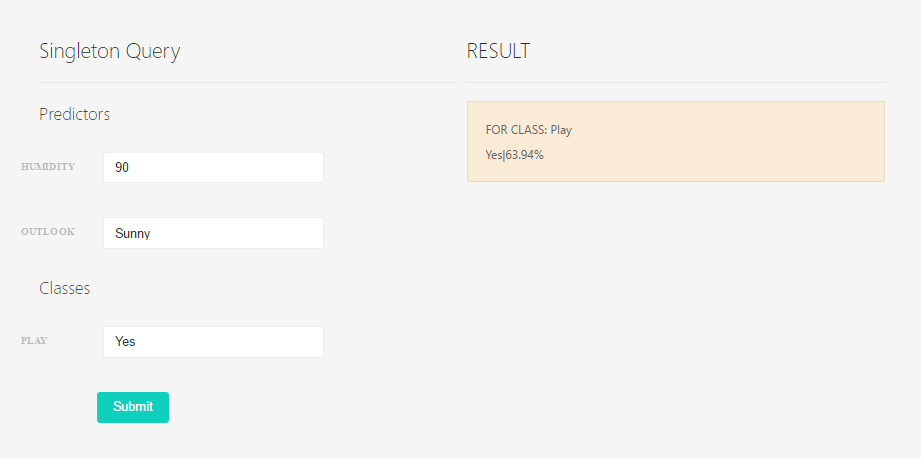
\includegraphics[scale=0.5]{Pengujian/result_classify_2}
	\caption[Hasil Klasifikasi Dataset-1]{Hasil Klasifikasi Dataset-2}
	\label{fig:Hasil Klasifikasi Dataset-2}
\end{figure}
	
\end{enumerate}

\subsection{Kesimpulan Pengujian Kebenaran}

Pada hasil yang pengujian yang telah dilakukan, dapat dibuktikan bahwa hasil perhitungan dengan menggunakan program dan manual memiliki hasil yang sama. Hanya saja angka presentase dominasi hasil yang dimiliki oleh program sedikit berbeda dengan angka presentase dominasi pada perhitungan manual. Untuk dataset pertama, pada perhitungan manual diperoleh hasil kelas \texttt{Play=Yes} dengan tingkat presentase dominasi sebesar \texttt{99.8\%}, sedangkan jika menggunakan program tingkat presentase dominasi-nya sebesar \texttt{100\%}. Untuk dataset pertama, pada perhitungan manual diperoleh hasil kelas \texttt{Play=Yes} dengan tingkat presentase dominasi sebesar \texttt{64\%}, sedangkan jika menggunakan program tingkat presentase dominasi-nya sebesar \texttt{63.94\%}. Perbedaan yang sangat kecil, yang berkisar diantara \texttt{0.02\% - 0.06\%} diperkirakan timbul karena pembulatan nilai desimal yang berbeda.

\section{Eksperimen}

\subsection{Pembuatan model}

\subsection{Performansi Big Data}